\chapter{Realization}
In the following chapter, we describe the realization of the software system. In section \ref{sec:structure}, we give an overview of the core components and how they interact with each other. 
In section \ref{sec:additional}, we describe additional components. Figure \ref{fig:componentsOverview} shows an overview of the core components. Additional components from section \ref{sec:additional} are omitted to prevent cluttering.

\begin{figure}[h]
    \centering
    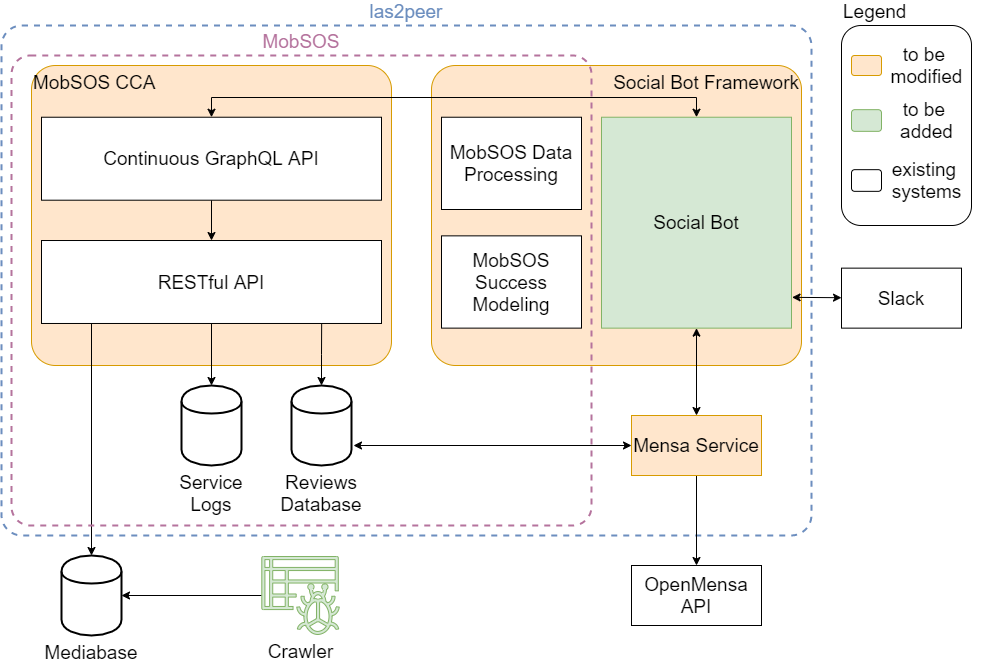
\includegraphics[width=\linewidth]{realization/components_overview.png}
    \caption{Overview of the different components}
    \label{fig:componentsOverview}
\end{figure}

\section{Structure}\label{sec:structure}
The system consists of three major components: the \emph{Social Framework}, the \emph{Mensa Service}\footnotemark and the \emph{MobSOS} services. 
% The resulting bot model can be seen in \ref{fig:botmodel}
\footnotetext{\href{https://github.com/rwth-acis/las2peer-Mensa-Service}{las2peer Mensa Service}}
\subsection{Social Bot Framework}
The Social Bot Framework is used to model and deploy the \emph{mensabot}. The mensabot is created in the space \emph{mensabot} of the Social Bot Framework.
% \begin{figure}[h]
%     \centering
%     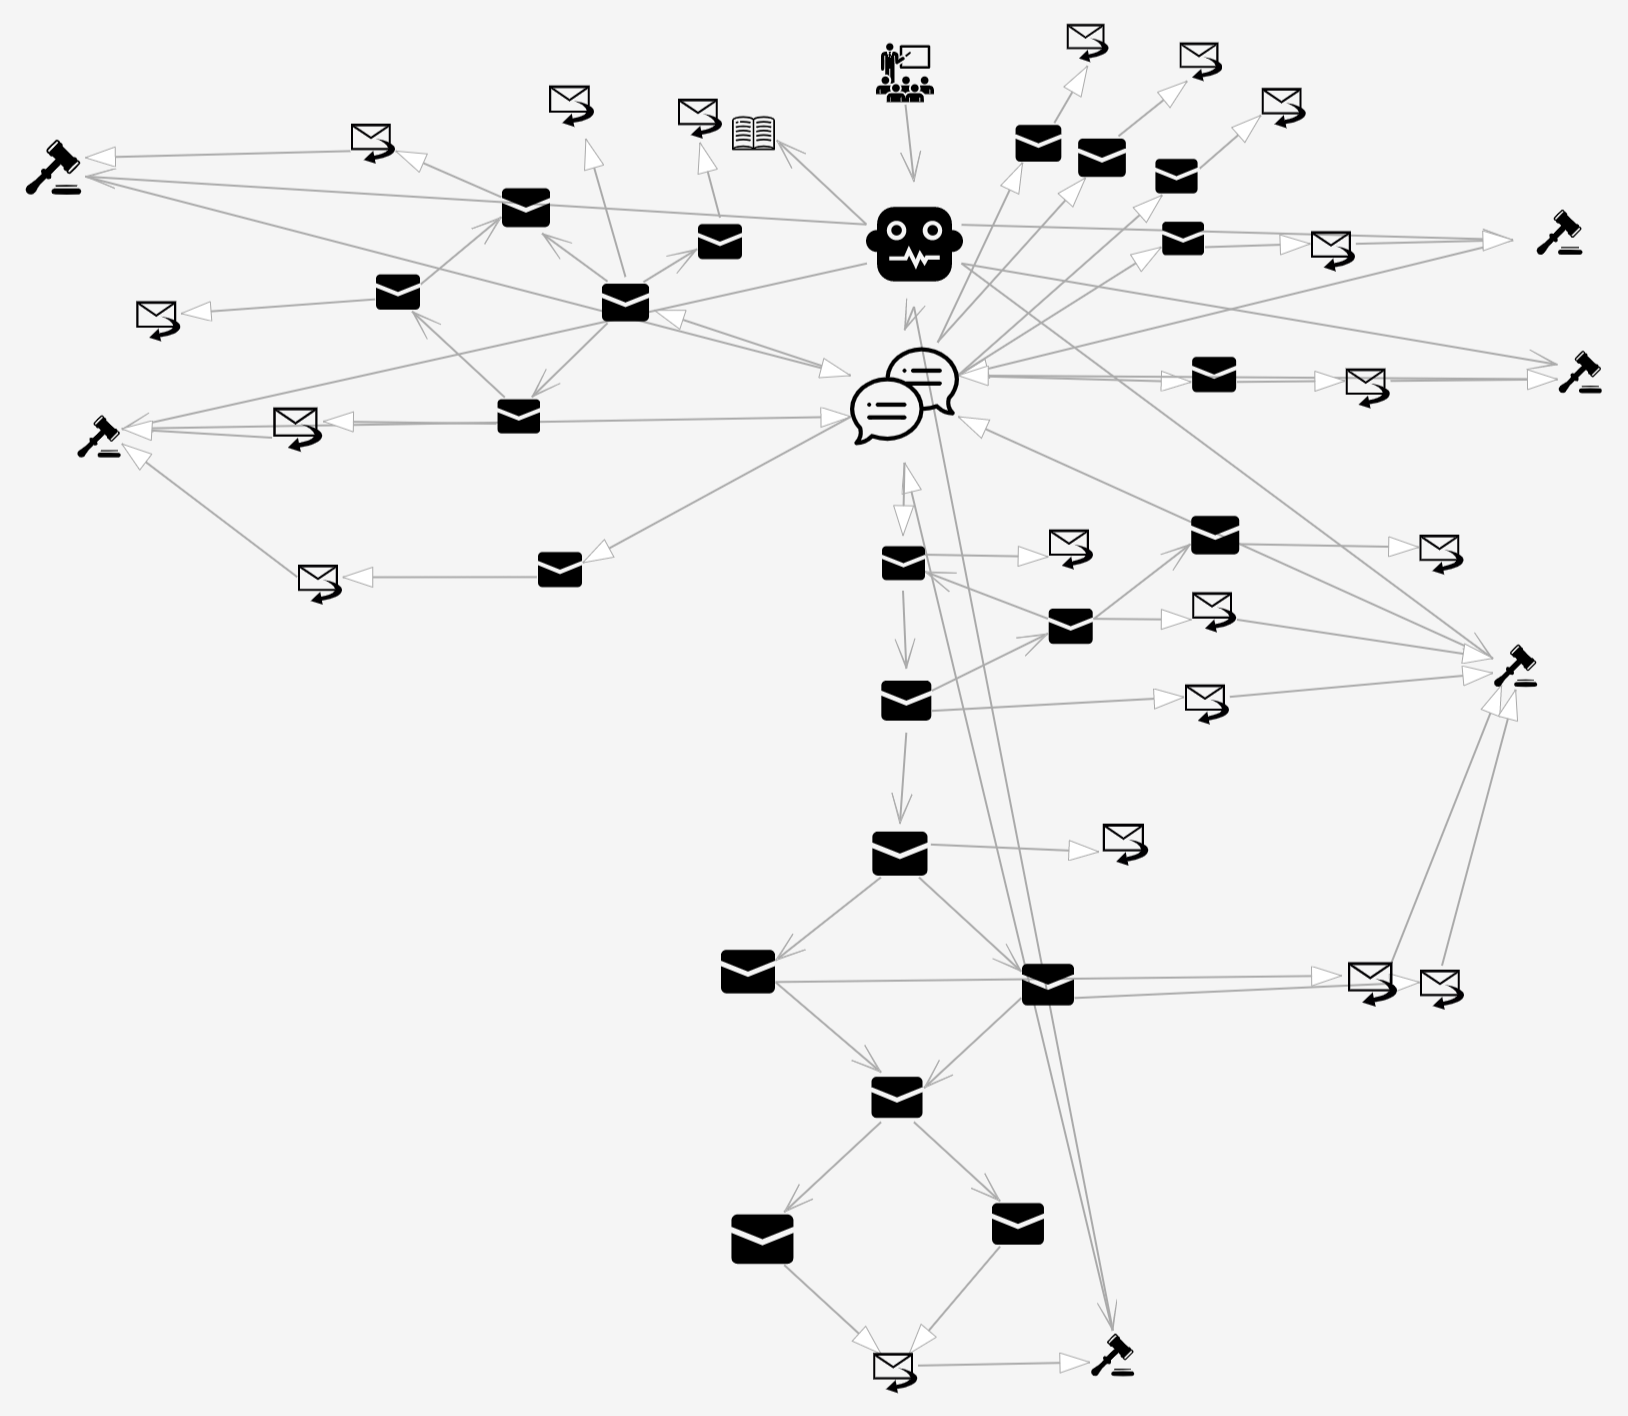
\includegraphics[width=\linewidth]{realization/botmodel.png}
%     \caption{Bot model inside the canvas}
%     \label{fig:botmodel}
% \end{figure}

The bot model is created on the canvas of the frontend. 
% The resulting model is shown in Figure \ref{fig:botmodel}. 
The frontend also serves to write the intents, which will be used to train an NLU model for intent recognition. 
The bot should be able to be added to group channels. The bot should act as a quiet agent listening to mentions and filter out the rest of the conversations.
A mention has the following form \texttt{@botname}, where \emph{botname} represents the username that the bot has in the Slack channel.


\subsection{MobSOS services}
The MobSOS services include the MobSOS Data Processing, MobSOS Success Modelling , MobSOS CCA GraphQL, MobSOS CCA REST services.

\subsubsection{MobSOS CCA GraphQL and REST}
The MobSOS CCA backend service has access to three different databases. First, the MobSOS CCA service can access the food reviews, which are stored inside the las2peer database of MobSOS.

Second, the system can access \emph{Mediabase} data, which contains data from reviews, made outside of the las2peer system. 
This data could be collected by a crawler bot, which searches Google and Twitter for reviews of the canteen. 
Those two databases provide mostly data for the Information Quality factors of the MobSOS success model.

Third, the service can also access monitoring data generated by the Bot and the Mensa Service, which are stored in the MobSOS database. 

Initially the REST service fetched data from the database by providing a SQL query and the database and schema on which it should run. It would then create a connection to that database, execute the query and create a JSON object from the \texttt{ResultSet}. 

The problem with this approach is that the order of the attributes, specified in the \texttt{SELECT} statement of the query, is lost.
However this order is crucial when making visualizations. 
Two possible solutions for this were taken into consideration:
\begin{enumerate}
    \item Modify the service to provide the data directly as an array of arrays.
    \item Send order information along with the response and then use that order information to sort the data.
\end{enumerate}
In order to still comply with the GraphQL specification, we went along with option 2. 

% Those monitoring messages provide the system quality factors of the MobSOS success model.



\subsubsection{MobSOS Success Modelling}

The measure definition was modified by including additional information about which database the query should be executed on. 
An example is shown in Listing \ref{lst:measure}.
The \texttt{data} element contains the SQL query under the \texttt{query} element and information about where to execute the query contained in the \texttt{database} element.
The attributes for the \texttt{database} element are \texttt{name} and \texttt{schema}. The name identifies the database on the GraphQL server. 
The schema describes which schema should be used.
If the database attribute is omitted, the default database name and schema are used, which are \texttt{las2peer} and \texttt{LAS2PEERMON} respectively.
This allows the community to visualize data from any database supported by the GraphQL service.

\begin{lstlisting}[language=XML, caption= example of a Measure, label=lst:measure,escapeinside={(*@}{@*)}]
<measure name="Your measurement">
    (*@\textcolor{blue}{<data name="Your dataset">}@*)   
        <query name="countOfMessage">
            SELECT COUNT(*) as number FROM MESSAGE
        </query>
        (*@\textcolor{blue}{<database name="las2peer" schema="LAS2PEERMON"/>}@*)
    (*@\textcolor{blue}{</data>}@*)
    <visualization type="Value">
        <unit/>
    </visualization>
</measure>
\end{lstlisting}

In the case of a chart visualization, the MobSOS Success Modelling service uses the Data2chart service. This service transforms the data into a picture of a chart in base64 encoding. This encoded picture is then sent back to the success modelling service which sends it back to the social bot manager.

\subsection{Data2Chart}
This service\footnotemark was written by us in order to render google charts as an image which could be sent to the chatbot and visualized in the chat. This service was created as an alternative to the MobSOS query visualization service which did not provide the option to render the chart as an image. 
\footnotetext{\url{https://github.com/lakhoune/image-renderer}}
The service is written in NodeJS and uses an NPM library called google-charts-node\footnotemark.
\footnotetext{\url{https://www.npmjs.com/package/google-charts-node}}
The google-charts-node module creates an html file which loads the google charts and then renders that html file in a headless browser \footnotemark and returns the resulting image.
\footnotetext{\url{https://www.npmjs.com/package/puppeteer}}
The MobSOS success modelling service calls the NodeJS server, if a bot is requesting a visualization. It includes the data for the graph in a \texttt{POST} request which has the following form:
\begin{lstlisting}
POST  http://localhost:3000/ HTTP/1.1
content-type: application/json

{
    "data": [...],
    "chartType":"BarChart",
    "options":{
        "title":"Chart title",
        "hAxis":{
            "title":"Axis title"
        }
    },
    "clean":true 
}
\end{lstlisting}
Under the data key, an array of data points. Each data point can be in the form of an array, or JSON object. 
The chartType specifies, the type of the chart. It uses the same format as the Google Charts API. 
Options also follow the same structure as defined by the Google Charts API.
The clean attribute specifies if the data should be cleaned. The Google Charts API expects each data point to be of the same length. Cleaning in this context means that each data point which has less attributes than the data point with the maximum number of attributes, is removed.
The data will be cleaned unless this attribute is specifically set to true.  

\subsection{Mensa Service}
The Mensa Service provides information about the community to the bot. This information includes: canteens, dishes and reviews. The Mensa service logs MobSOS data which is later used to get insights about how the Mensa community uses the service.

The Mensa service was also extended to use the OpenMensa API \footnote{\url{https://openMensa.org/}}. 
Using the OpenMensa API has one drawback. The menu is displayed only in the local language of the canteen, so we cannot get the dishes name in English anymore.
However it also has many advantages:
\begin{itemize}
    \item We are not limited to canteens in Aachen, but can get canteens from all over Germany, Luxembourg and Austria. 
    \item We do not have to scrape the  webpage of the Studierendenwerk \footnote{\href{https://www.studierendenwerk-aachen.de/}{Studierendenwerk Aachen}}, which is prone to errors if they change their frontend.
\end{itemize}
Initially the service stored canteen related information in the shared node storage. The service was modified to use its own database. Using a database allows us to persist data and make them available for MobSOS related success visualizations. 
Therefore some tables were added to the LAS2PEERMON schema:
\begin{itemize}
    \item \texttt{Mensas}: This table contains information about canteens, supported by the OpenMensa API. It contains the columns:
    \begin{itemize}
        \item id (int PK): The id of the canteen
        \item name (varchar(255)): The name of the canteen
        \item address (varchar(255)): The address of the canteen
        \item city (varchar(255)): The city in which the canteen is located 
    \end{itemize}
    The entries are updated once a month, as the list of canteens does not change often \footnote{\href{ OpenMensa API specification}{https://doc.openmensa.org/api/v2/canteens/}}
    \item \texttt{Dishes}: This table contains information about the dishes served at canteens. It is updated whenever a menu is fetched for a canteen which had not been fetched in the last six hours. It contains the following columns:
    \begin{itemize}
        \item id (int PK): The id of the dish. 
        \item mensaId (int PK): The id of the canteen at which the dish was served. The id references a key in the \texttt{mensas} table
        \item name (varchar(255)): The name of the dish.
        \item category (varchar(255)): The category of the dish. Categories do not seem to be structured, each region of canteen seems to have their own category names
    \end{itemize}
    \item \texttt{Reviews}: This table contains reviews of food made by the community. It contains the following columns:
    \begin{itemize}
        \item id (int AI PK): The id of the review.
        \item author (varchar(255)): The  author of the review. For reviews made by the chatbot, the email address of the user is used.
        \item mensaId (int): The id of the canteen at which the food was served. This attribute references a canteen in the \texttt{mensas} table
        \item dishId (int): The id of the dish. This id references a dish in the \texttt{dishes} table.
        \item timestamp (timestamp): The timestamp at which the review was recorded
        \item stars (int): The overall satisfaction with the food. The values range from 1 to 5.
        \item comment (varchar(255)): The user can choose to add a comment to his review.
    \end{itemize}
\end{itemize}
The tables were added to the LAS2PEERMON schema, but in the future it could be setup as its own seperate Mediabase.
Ids seem to be unique for each dish at each canteen, each day it is served. To reduce overhead we should define name, mensaId as primary keys for dishes.


\section{Social Bot}

The bot acts as an interface between the user, and the las2peer backend services. The bot is called \emph{Mensabot}.
Chat messages from users are sent to the bot manager service. 
The bot manager uses a RASA server for intent recognition. 
The RASA server also extracts the name of the Mensa and the city in which it is located as possible intent entities from the user input.

Certain actions, like requesting the menu or a visualisation , trigger a service call to the \emph{Mensa Service}, or the \emph{Success Modelling Service}.
The services get access to the user message.  
The services also get access to context information like the intent and the entities that were recognized by the RASA server.

Furthermore they also get access to meta-information from the chat platform like the \texttt{channel\_id} of the Slack channel or the email address of the chat user. 
The email address is used to store user information in the service. This is done in a static HashMap, which maps email addresses to context information. The context information for a particular user is a \texttt{JSON} object containing itself generic \texttt{Object}s referenced by a \texttt{string} key. 
Storing this information inside the service is important for a REST service, as the context will not be provided on a next service request.

\subsection{Communication with the Mensa Service}
The first feature, which was implemented was querying the menu for a specific canteen. 
The process is depicted in Figure \ref{fig:getMenu}.
\begin{figure}[h]
    \centering
    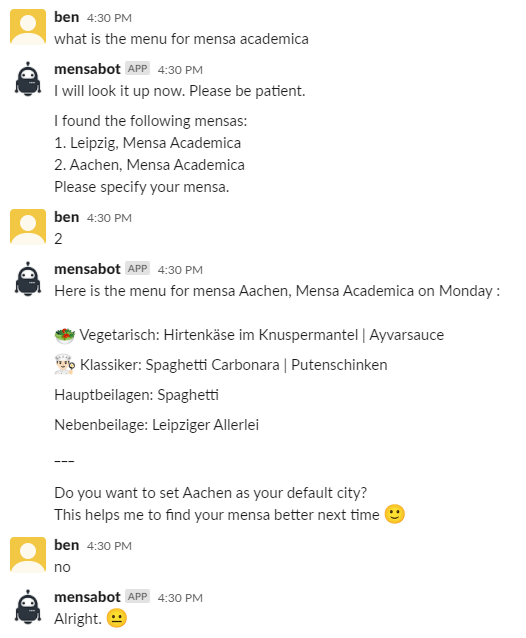
\includegraphics[width=8cm]{realization/bot/menu.png}
    \caption{Get canteen related information}
    \label{fig:getMenu}
\end{figure}
The user asks the bot for the menu at a specific canteen, which results in a \emph{Bot Action} being triggered. This action calls the las2peer Mensa service. 

Possible intent entities which are recognized at this step are the \emph{name} of the canteen and the \emph{city} in which the canteen is located.
If the name of the canteen is not recognized, the bot will ask  the user again to specify it. 

The city name can be omitted. In this case it is possible that multiple canteens match the name provided by the user. I that case, the bot will provide a list of all matching canteen names and then ask the user to choose one of the canteens from the list. The list is saved in context, so that the user can provide a number and the service can then select the appropriate canteen from the list.

After fetching the menu the bot asks the user if they would like to set the city in which the canteen is located as their default city. If the user types yes, then this city is saved in the context of the user. On further requests this information can be helpful to extract the right canteen if more canteen names are possible. 
We chose to set the default city instead of the default canteen students from one Mensa community might visit different canteens in the same city and less likely to change cities. 

Next the review process was implemented as a question-based dialogue. An example can be seen in figure \ref{fig:addReview}.

% \begin{figure}[h]
%     \centering
%     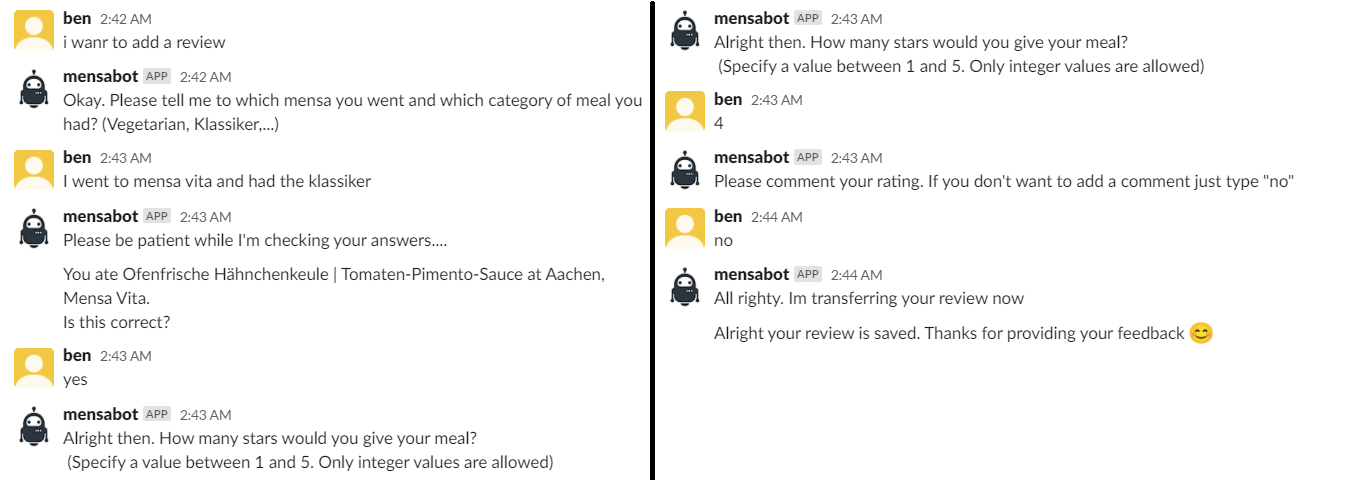
\includegraphics[width=\linewidth]{realization/bot/review.png}
%     \caption{Add a review}
%     \label{fig:addReview}
% \end{figure}

\begin{figure}[h]
    \begin{minipage}{0.5\textwidth}
        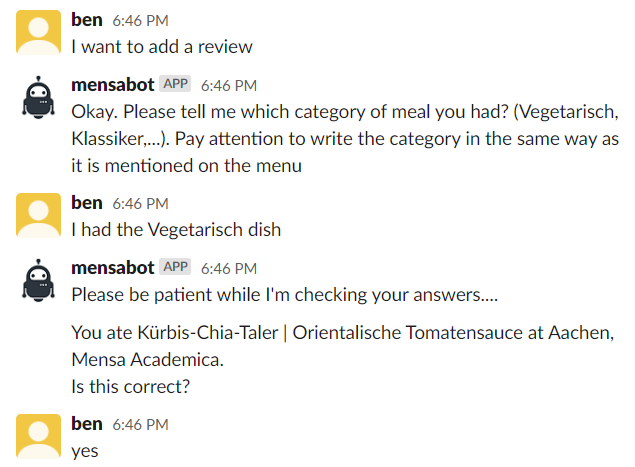
\includegraphics[width=\textwidth]{realization/bot/review1.png} 
    \end{minipage}
    \begin{minipage}{0.5\textwidth}
        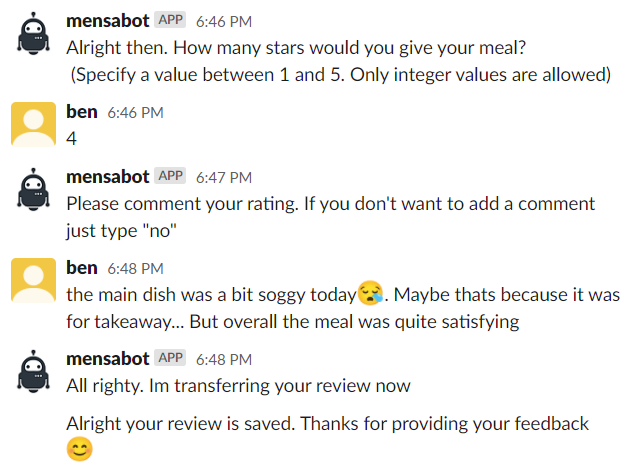
\includegraphics[width=\textwidth]{realization/bot/review2.png}
        
    \end{minipage}
    \caption{An example of what the review process looks like}
    \label{fig:addReview}
\end{figure}

The bot starts by asking the user to which canteen the user went to and what category of dish they had. If the user did not specify a canteen, but had previously asked for the menu, then the Mensa service gets the canteen from the \texttt{ContextInfo}. 

The available intent entities are the name of the canteen and the category of dish (e.g. Klassiker/ Vegetarisch).
The bot then extracts the dish from the menu and asks the user if the canteen and dish were correctly selected. 
Currently, dishes are only extracted by dish category, by using simple string matching. Furthermore, the dish categories need to be provided in the same way that they are mentioned on the menu. In our case, this means that they need to be provided in German.

If the user confirms the selection then the process continues. 
The canteen and dish are stored in the context. 
If the selection was wrong the bot asks the user to retry specifying the canteen and dish. 
The context is reset to the previous step in this case, this also includes removing the dish and canteen from the user context in the service.

After the user has confirmed that the right canteen and dish were indeed selected, the bot continues to ask the user how many stars (between 1 and 5) the user would give their meal. 
The bot asks the user to add a comment to the review. The user may or not add a comment. If the user types \emph{no} into the chat the bot recognizes this as a rejection intent and adds a review without comment.

Both of these features were be implemented first, as this allowed us to start collecting food reviews and service logs, which can then be evaluated at a later time with the Success Modelling service.
Making food reviews should only be allowed in private chat with the bot. 
The menu query should be available both in private chat and in channels.
For this to work the Social Bot Manager service needs to be updated so that it can discern between private and public channels.

\subsection{Communication with the MobSOS Success Modelling service}

The next feature, which was implemented was the visualisation of success measures. Users can request them by stating that they want to visualize something.
This triggers the visualization routine of the bot. Figure \ref{fig:visualReqSeq} shows how different components are used in a visualization.
\begin{figure}[h]
    \centering
    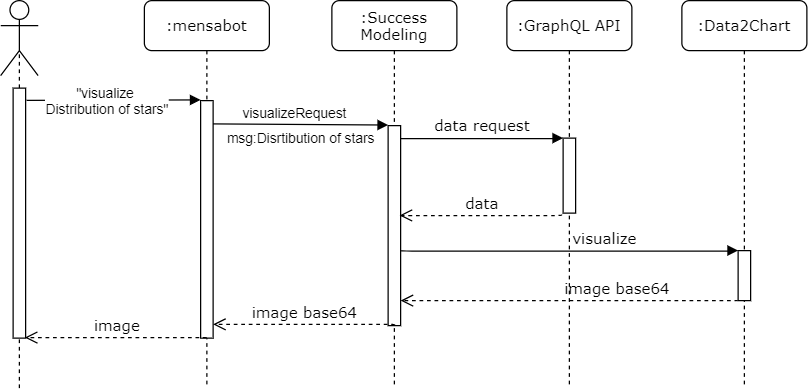
\includegraphics[width=\linewidth]{realization/visualization_sequence.png}
    \caption{Sequence diagram of a visualization request}
    \label{fig:visualReqSeq}
\end{figure}

The bot starts by asking providing the name of a success \emph{measure}. Alternatively the user can also ask the bot to list all measures of the success model.
If the user asked to list measures, they can then choose one of the measure name from the list. 
The measure name is passed on to the Success Modelling service. The service then gets the success model for the community. In our case this is done by using the default group name and default service name, but they can be specified too.
If a group different to the default group is chosen, then the service checks if the chat user is part of the las2peer group. 
It is important to note here that the email address needs to be assigned to an Agent in the network. 
This can be done by using the las2peer frontend. 
Groups can also be managed under \emph{AgentTools} on the frontend.  
The service looks up the measure in the measure catalog. The desired measure is chosen by matching the name with the name the user provided. 
The resulting visualization is sent back to the bot service. If the visualization is a chart, the chart is sent as an base64 encoded image.

If no name was found, the service looks up measures which have tags contained in the user input. The results from the tag-search are returned to the user and the user can choose the measure which they want to visualize.
An example can be seen in figure \ref{fig:visualReq}.
% \begin{figure}[h]
%     \centering
%     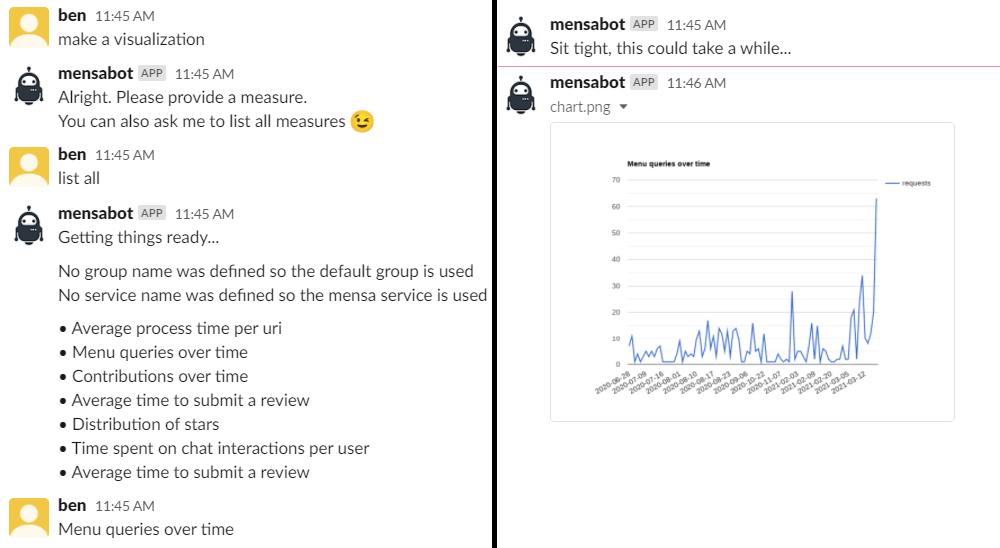
\includegraphics[width=\linewidth]{realization/bot/visual.png}
%     \caption{Requesting a visualisation}
%     \label{fig:visualReq}
% \end{figure}

\begin{figure}[h]
    \begin{minipage}[t]{0.5\textwidth}
        \centering
\vspace{0pt}

        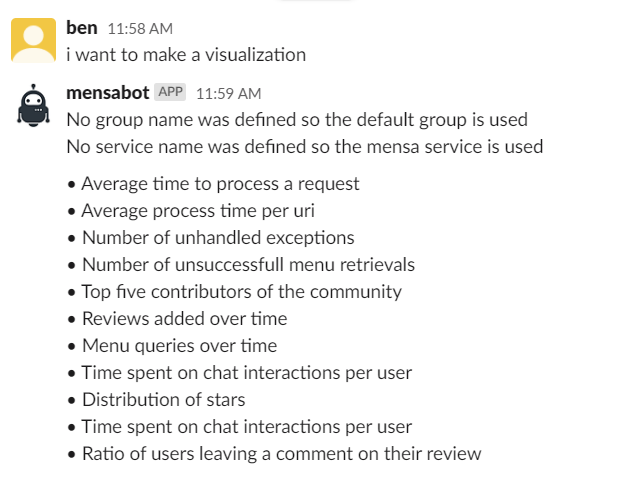
\includegraphics[width=\textwidth]{realization/bot/visual1.png} 
    \end{minipage}
    \begin{minipage}[t]{0.5\textwidth}
        \centering
\vspace{0pt}

        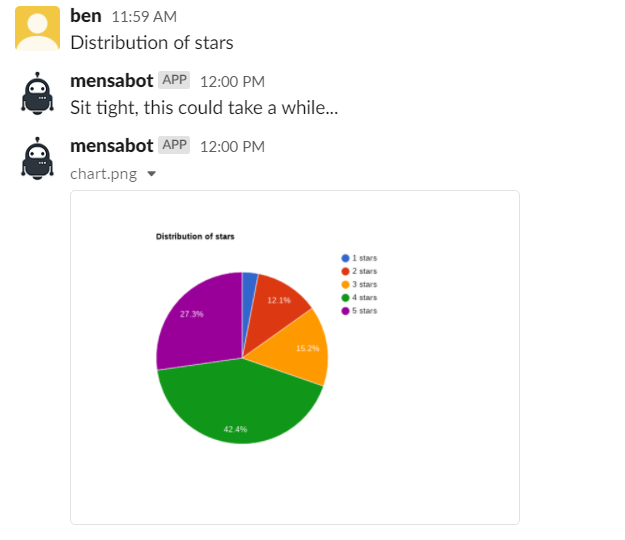
\includegraphics[width=\textwidth]{realization/bot/visual2.png}
    \end{minipage}
    \caption{An example of what the review process looks like}
    \label{fig:visualReq}
\end{figure}


The final feature, which was implemented is editing the success model. The user first needs to state that he wants to update the success model of the community.
Currently, elements cannot be updated. 
However they can be deleted or added. 
To delete a factor or a measure, the user specifies it as follows \begin{lstlisting}
    remove <factor/measure> [name]
\end{lstlisting}  
Adding a measure is a bit more complicated. The user first selects a \emph{dimension} which they want to add a measure to. The user then specifies the \emph{factor} under which the measure will be appended. The user can also add a factor by providing a new name. Finally the user chooses one of the measures from the catalog to add it to the success model. 
The measures from the catalog are predefined using a tool like the MobSOS Evaluation Center. 

After discussions with my supervisor, we decided not to add the ability to formulate queries directly with the bot. 
We argue that this is not a crucial requirement, because community members might not necessarily know how to write them. Furthermore, the ones that do, can probably do it more efficiently by editing the measure catalog directly.

% The measures contain a \texttt{tags} attribute which can be used to add keywords to a measure. The bot uses entity extraction to extract possible tags from a user message, which then are used in the success modelling service to find the right measure for the visualization in the measure catalog and success model.

% The Bot Service communicates with the MobSOS Success Modelling system in order to get visualisations of the success model. The bot sends the resulting visualisations to the user in chat.
% Furthermore, it can also be used to modify the success model of the community. 
% Finally the success modelling will be implemented. Users should be able
% to modify the success model in chat. Therefore, an update routine needs to be implemented, which is started at the recognition of a specific intent.
% The bot is modelled with the help of the Social Bot Framework frontend canvas and deployed on the las2peer social bot manager service.


\section{Additional services}\label{sec:additional}
Some additional systems were deployed or added during my work.

\subsection{Mensa Guide}
The Mensa Guide service is a frontend to the las2peer Mensa service. It provides basic functionalities like getting the menu for canteens in Aachen, making reviews and uploading pictures for dishes. It was updated to use latest version of the Mensa service backend. It should also be extended in the future to use all available canteens. This should be easy to do as we have added a service function to get a list of all canteens in a particular city.

\subsection{MobSOS evaluation Center}
The MobSOS evaluation Center is a service which communicates with the MobSOS backend services. It provides a range of functionalities. Those include: contact management and group management. 
It also allows community members to edit existing success models or create new ones.
Furthermore it also provides visualizations for the measures of the success model, which it gets from the MobSOS query visualization service.

\subsection{MobSOS query visualization service}
The MobSOS query visualization service is a las2peer service which can be used to make visualizations of data in a database. It also allows users to add new database and store SQL queries. The MobSOS Evaluation Center uses this service to get the visualizations for success measures.

% \subsection{MobSOS CCA}
% The MobSOS CCA system needs to be extended such that the success model data can be visualized and sent as a picture to the user. Therefore, the Google Charts API will be used in combination with an HTML renderer, which will render the visualizations which were produced by the Charts API and send them back as a PNG to the Bot Service.

% This measure is recognized by the bot to run the visualisations. Additionally, templates will be available, which are to be run when specific intents are recognized, such that the query visualisations can be done in an intuitive way.

% \begin{figure}
%     \centering
%     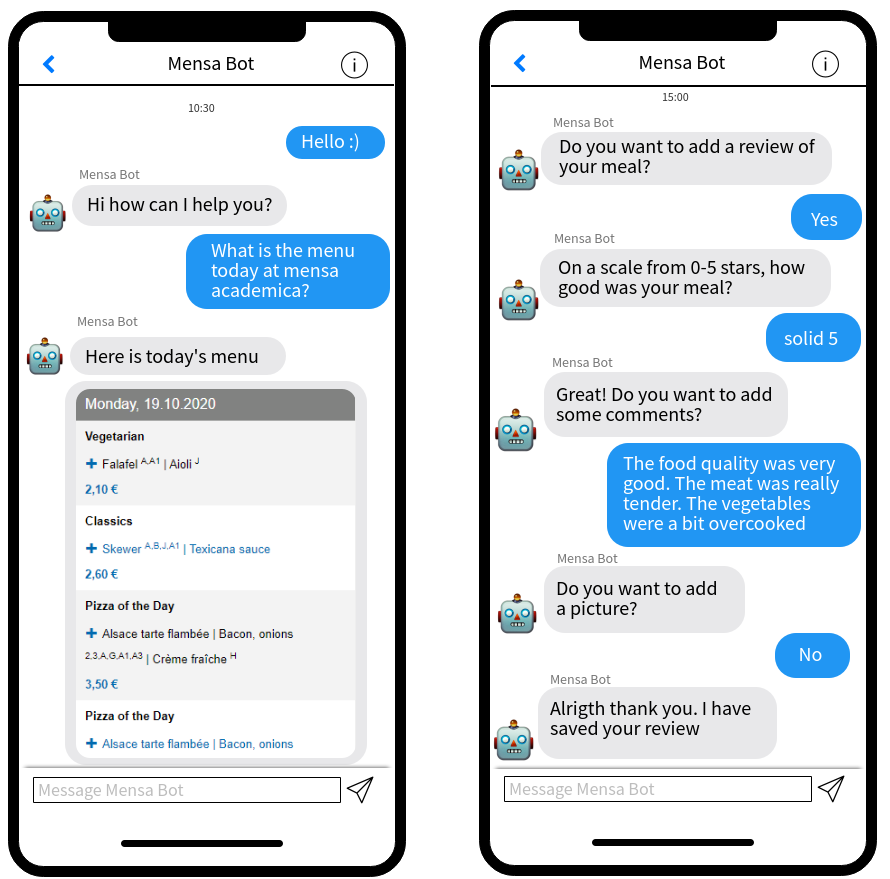
\includegraphics[height=0.45\textheight]{realization/chat_mockup.png}
%     \caption{Example use of community Service with the Bot}
%     \label{fig:chatMockup}
% \end{figure}

% \begin{figure}
%     \centering
%     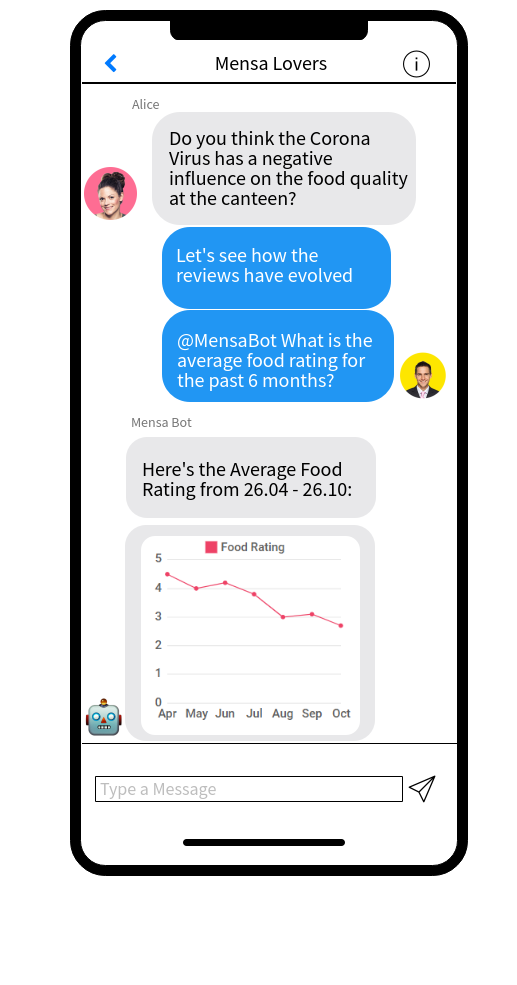
\includegraphics[height=0.45\textheight]{realization/visual_req.png}
%     \caption{Example of a chat interaction with the Bot}
%     \label{fig:visualReq}
% \end{figure}